% Unofficial University of Cambridge Poster Template
% https://github.com/andiac/gemini-cam
% a fork of https://github.com/anishathalye/gemini
% also refer to https://github.com/k4rtik/uchicago-poster

\documentclass[final]{beamer}

% ====================
% Packages
% ====================

\usepackage[T1]{fontenc}
\usepackage{lmodern}
\usepackage[size=custom,width=120,height=72,scale=1]{beamerposter}
\usetheme{gemini}
\usecolortheme{cam}
\usepackage{graphicx}
\usepackage{booktabs}
\usepackage[numbers]{natbib}
\usepackage{tikz}
\usepackage{pgfplots}
\pgfplotsset{compat=1.14}
\usepackage{anyfontsize}
\usepackage{tcolorbox}
\usepackage{lipsum} % Package for Lorem Ipsum

\usepackage{amsmath}  % For mathematical equations
\usepackage{amssymb}  % For additional mathematical symbols
\usepackage{bm}       % For bold math symbols
\usepackage{cite}     % For citations (optional)

\usepackage{caption}  % For caption formatting
\usepackage{subcaption} % For subfigures (optional


\usetikzlibrary{shapes.geometric, arrows}

% ====================
% Lengths
% ====================

% If you have N columns, choose \sepwidth and \colwidth such that
% (N+1)*\sepwidth + N*\colwidth = \paperwidth
\newlength{\sepwidth}
\newlength{\colwidth}
\setlength{\sepwidth}{0.025\paperwidth}
\setlength{\colwidth}{0.3\paperwidth}

\newcommand{\separatorcolumn}{\begin{column}{\sepwidth}\end{column}}

\newtcolorbox[auto counter, number within=section]{highlightbox}[2][]{%
    colback=yellow!20, % Background color
    colframe=red!50!black, % Border color
    fonttitle=\bfseries, % Bold title
    title={#2}, % Title of the box
    #1 % Additional options
}

\newtcolorbox[auto counter, number within=section]{infobox}[2][]{%
    colback=blue!10!white, % Background color
    colframe=blue!80!black, % Border color
    fonttitle=\bfseries, % Bold title
    title={#2}, % Title of the box
    #1 % Additional options
}

% ====================
% Title
% ====================

\title{Improved Denoising Diffusion Probabilistic Models​}

\author{Gloria Sun \inst{1} \and Hung Phan Huy \inst{1} \and Jack Clarkson \inst{1}}

\institute[shortinst]{\inst{1} University of Cambridge, Department of Engineering}

% ====================
% Footer (optional)
% ====================

\footercontent{
  \href{https://www.example.com}{https://www.example.com} \hfill
  ABC Conference 2025, New York --- XYZ-1234 \hfill
  \href{mailto:alyssa.p.hacker@example.com}{alyssa.p.hacker@example.com}}
% (can be left out to remove footer)

% ====================
% Logo (optional)
% ====================

% use this to include logos on the left and/or right side of the header:
% \logoright{\includegraphics[height=7cm]{logo1.pdf}}
% \logoleft{\includegraphics[height=7cm]{logo2.pdf}}

% ====================
% Body
% ====================

\begin{document}

% Refer to https://github.com/k4rtik/uchicago-poster
% logo: https://www.cam.ac.uk/brand-resources/about-the-logo/logo-downloads
\addtobeamertemplate{headline}{}
{
	\begin{tikzpicture}[remember picture,overlay]
		\node [anchor=north west, inner sep=3cm] at ([xshift=0.0cm,yshift=1.0cm]current page.north west)
		{\includegraphics[height=4.5cm]{logos/cambridge-reversed-color-logo.eps}};
	\end{tikzpicture}
}

\begin{frame}[t]
	\begin{columns}[t]
		\separatorcolumn

		\begin{column}{\colwidth}

			\begin{block}{Denoising Diffusion Probabilistic Models (DDPM)}
				Diffusion models are parameterized Markov chains trained using variational inference to produce samples matching the distribution of input images after finite time. 
				They are latent variable models of the form \( p_{\theta}(\mathbf{x}_0) := \int p_{\theta}(\mathbf{x}_{0:T}) \, d\mathbf{x}_{1:T} \), where \( \mathbf{x}_1, \dots, \mathbf{x}_T \) are latents of the same dimensionality as the data \( \mathbf{x}_0 \sim q(\mathbf{x}_0) \). 
				
				% \vspace{5pt}
				
				\begin{infobox}{Forward Process}
					The model consists of a \textit{forward process} $q(\mathbf{x}_{1:T} \mid \mathbf{x}_0)$ which produces the latents by adding Gaussian noise at each timestep $t$ with variance $\beta_{t} \in (0, 1)$:
					
					\begin{equation}
						q(\mathbf{x}_{1:T} | \mathbf{x}_0) := \prod_{t=1}^{T} q(\mathbf{x}_t | \mathbf{x}_{t-1}), 
						\quad 
						q(\mathbf{x}_t | \mathbf{x}_{t-1}) := \mathcal{N}(\mathbf{x}_t; \sqrt{1 - \beta_t} \mathbf{x}_{t-1}, \beta_t \mathbf{I})
					\end{equation}

					If $T$ is sufficiently large and the schedule of $\beta_t$ is well behaved, $x_{T}$ will converge to an isotropic Gaussian distribution. If we know the exact reverse distribution $q(x_{t-1} \mid x_{t})$, we can sample $x_T \sim \mathcal{N}(0, \mathbf{I})$ and iteratively compute exact reverse distribution to get a sample from $q_{0}(x_{0})$. However, $q(x_{t-1} | x_{t})$ depends on the entire data distribution meaning it's intractable. We can approximate it using a neural network to get $p_\theta(x_{0:T})$, the \textit{reverse process}.
				\end{infobox}

				\begin{infobox}{Reverse Process}
					The joint $p_\theta(x_{0:T})$ defines the \textit{reverse process} which is a Markov chain with learned Gaussian transitions starting at $p(x_{T}) = \mathcal{N}(x_{t}; \mathbf{0}, \mathbf{I})$.
					\begin{equation}
						p_{\theta}(\mathbf{x}_{0:T}) := p(\mathbf{x}_T) \prod_{t=1}^{T} p_{\theta}(\mathbf{x}_{t-1}|\mathbf{x}_t),
						\quad
						p_{\theta}(\mathbf{x}_{t-1}|\mathbf{x}_t) := \mathcal{N}(\mathbf{x}_{t-1}; \boldsymbol{\mu}_{\theta}(\mathbf{x}_t, t), \boldsymbol{\Sigma}_{\theta}(\mathbf{x}_t, t))
					\end{equation}
				\end{infobox}

			\end{block}

			The model parameters $\mu_\theta$ and $\Sigma_\theta$ in the reverse process are trained using a neural network to denoise the images by optimising the variational bound on the negative log likelihood, given by:
			\begin{equation}
				\mathbb{E}_q\left[\underbrace{KL(q(x_T\vert x_0) \vert\vert p(x_T))}_{L_T} + \sum_{t> 1}\underbrace{KL(q(x_{t-1}\vert x_t, x_0)\vert\vert p_{\theta}(x_{t-1}\vert x_t))}_{L_{t-1}} - \underbrace{\log p_{\theta}(x_0 \vert x_1)}_{L_0}\right] = L
			\label{eq:nll1}
			\end{equation}
			

			% \begin{columns}[t] % Second row (Side-by-side blocks)

			% 	% First side-by-side block
			% 	\begin{column}{0.48\textwidth}
			% 		\begin{block}{Forward Process}
			% 			The forward process adds Gaussian noise:
			% 			\vspace{4pt}
			% 			\[
			% 				q(\mathbf{x}_{1:T} \mid \mathbf{x}_0) := \prod_{t=1}^{T} q(\mathbf{x}_t \mid \mathbf{x}_{t-1})
			% 			\]
			% 			\vspace{2pt}
			% 			\[
			% 				q(\mathbf{x}_t \mid \mathbf{x}_0) = \mathcal{N}(\mathbf{x}_t; \sqrt{\bar{\alpha}_t} \mathbf{x}_0, (1 - \bar{\alpha}_t) \mathbf{I})
			% 			\]
			% 			\vspace{4pt}where \( \bar{\alpha}_t = \prod_{s=1}^{t} (1 - \beta_s) \). This transforms data into a Gaussian prior for the reverse process.

			% 		\end{block}
			% 	\end{column}

			% 	% Second side-by-side block
			% 	\begin{column}{0.48\textwidth}
			% 		\begin{block}{Reverse Process}
			% 			The reverse process reconstructs data via a learned Gaussian transition:
			% 			\vspace{2pt}
			% 			\[
			% 				p_{\theta}(\mathbf{x}_{t-1} \mid \mathbf{x}_t) = \mathcal{N}(\mathbf{x}_{t-1}; \mu_{\theta}(\mathbf{x}_t, t), \Sigma_{\theta}(\mathbf{x}_t, t))
			% 			\]
			% 			\vspace{2pt}where \( \mu_{\theta}(\mathbf{x}_t, t) \) is estimated using a neural network \( \epsilon_{\theta}(\mathbf{x}_t, t) \) trained to predict noise.

			% 		\end{block}
			% 	\end{column}

			% \end{columns}

			\begin{block}{Model Outputs: Progressive Generation}

				\begin{figure}[h]
					\centering
					\begin{minipage}{0.6\textwidth}
						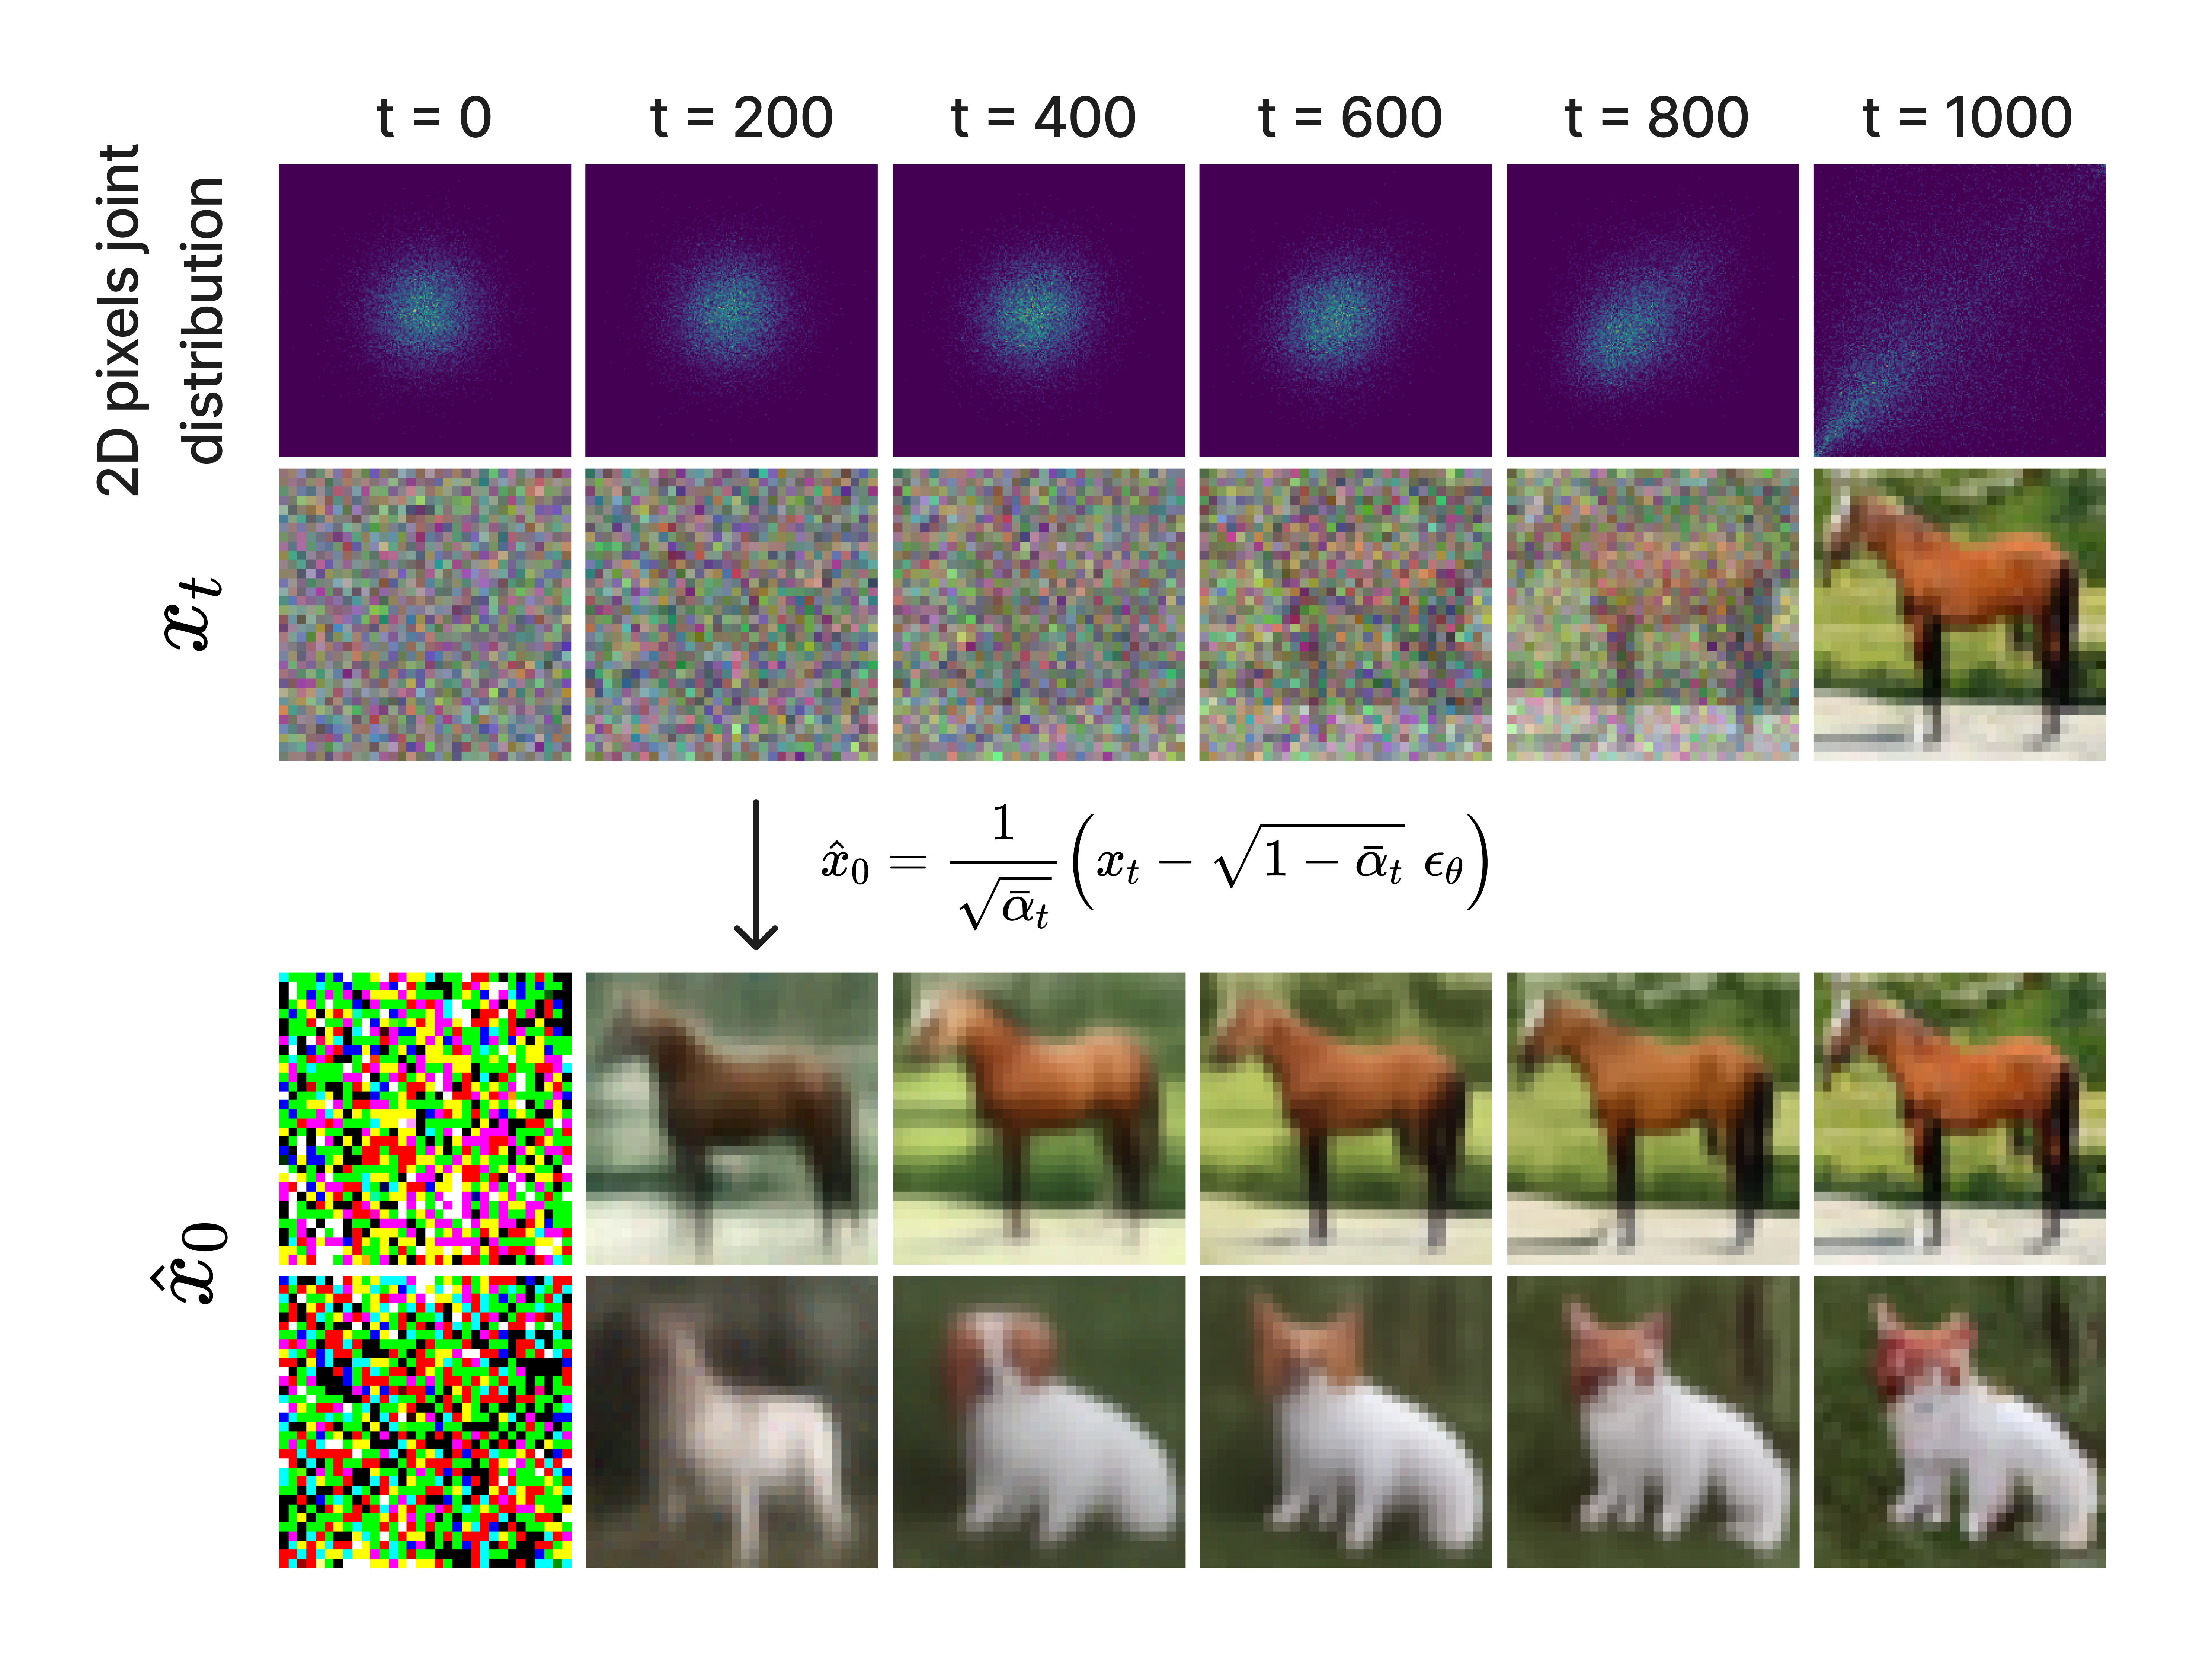
\includegraphics[width=\linewidth]{figs/model_outputs.png}
						\caption{Progressive generation of unconditional CIFAR-4 model, showing $x_{t}$, its joing density between 2 pixels, and the corresponding $\hat{x_{0}}$ over the reverse sampling steps.}
					\end{minipage}%
					\begin{minipage}{0.4\textwidth}
						\textbf{Description:} This figure shows the output of our model after training. The generated samples illustrate the learned distribution and denoising process over time. Key observations include:
						\begin{itemize}
							\item Sample diversity increases with more training.
							\item Noise reduction is evident in later timesteps.
							\item Model captures realistic patterns.
						\end{itemize}
					\end{minipage}
				\end{figure}

			\end{block}

			% \begin{alertblock}{A highlighted block}

			% 	This block catches your eye, so \textbf{important stuff} should probably go
			% 	here.

			% 	Curabitur eu libero vehicula, cursus est fringilla, luctus est. Morbi
			% 	consectetur mauris quam, at finibus elit auctor ac. Aliquam erat volutpat.
			% 	Aenean at nisl ut ex ullamcorper eleifend et eu augue. Aenean quis velit
			% 	tristique odio convallis ultrices a ac odio.

			% 	\begin{itemize}
			% 		\item \textbf{Fusce dapibus tellus} vel tellus semper finibus. In
			% 		      consequat, nibh sed mattis luctus, augue diam fermentum lectus.
			% 		\item \textbf{In euismod erat metus} non ex. Vestibulum luctus augue in
			% 		      mi condimentum, at sollicitudin lorem viverra.
			% 		\item \textbf{Suspendisse vulputate} mauris vel placerat consectetur.
			% 		      Mauris semper, purus ac hendrerit molestie, elit mi dignissim odio, in
			% 		      suscipit felis sapien vel ex.
			% 	\end{itemize}

			% 	Aenean tincidunt risus eros, at gravida lorem sagittis vel. Vestibulum ante
			% 	ipsum primis in faucibus orci luctus et ultrices posuere cubilia Curae.

			% \end{alertblock}

		\end{column}

		\separatorcolumn

		\begin{column}{\colwidth}

			\begin{block}{Improving the Noise Schedule}

				Vivamus congue volutpat elit non semper. Praesent molestie nec erat ac
				interdum. In quis suscipit erat. \textbf{Phasellus mauris felis, molestie
					ac pharetra quis}, tempus nec ante. Donec finibus ante vel purus mollis
				fermentum. Sed felis mi, pharetra eget nibh a, feugiat eleifend dolor. Nam
				mollis condimentum purus quis sodales. Nullam eu felis eu nulla eleifend
				bibendum nec eu lorem. Vivamus felis velit, volutpat ut facilisis ac,
				commodo in metus.

				\begin{figure}[h]
					\centering
					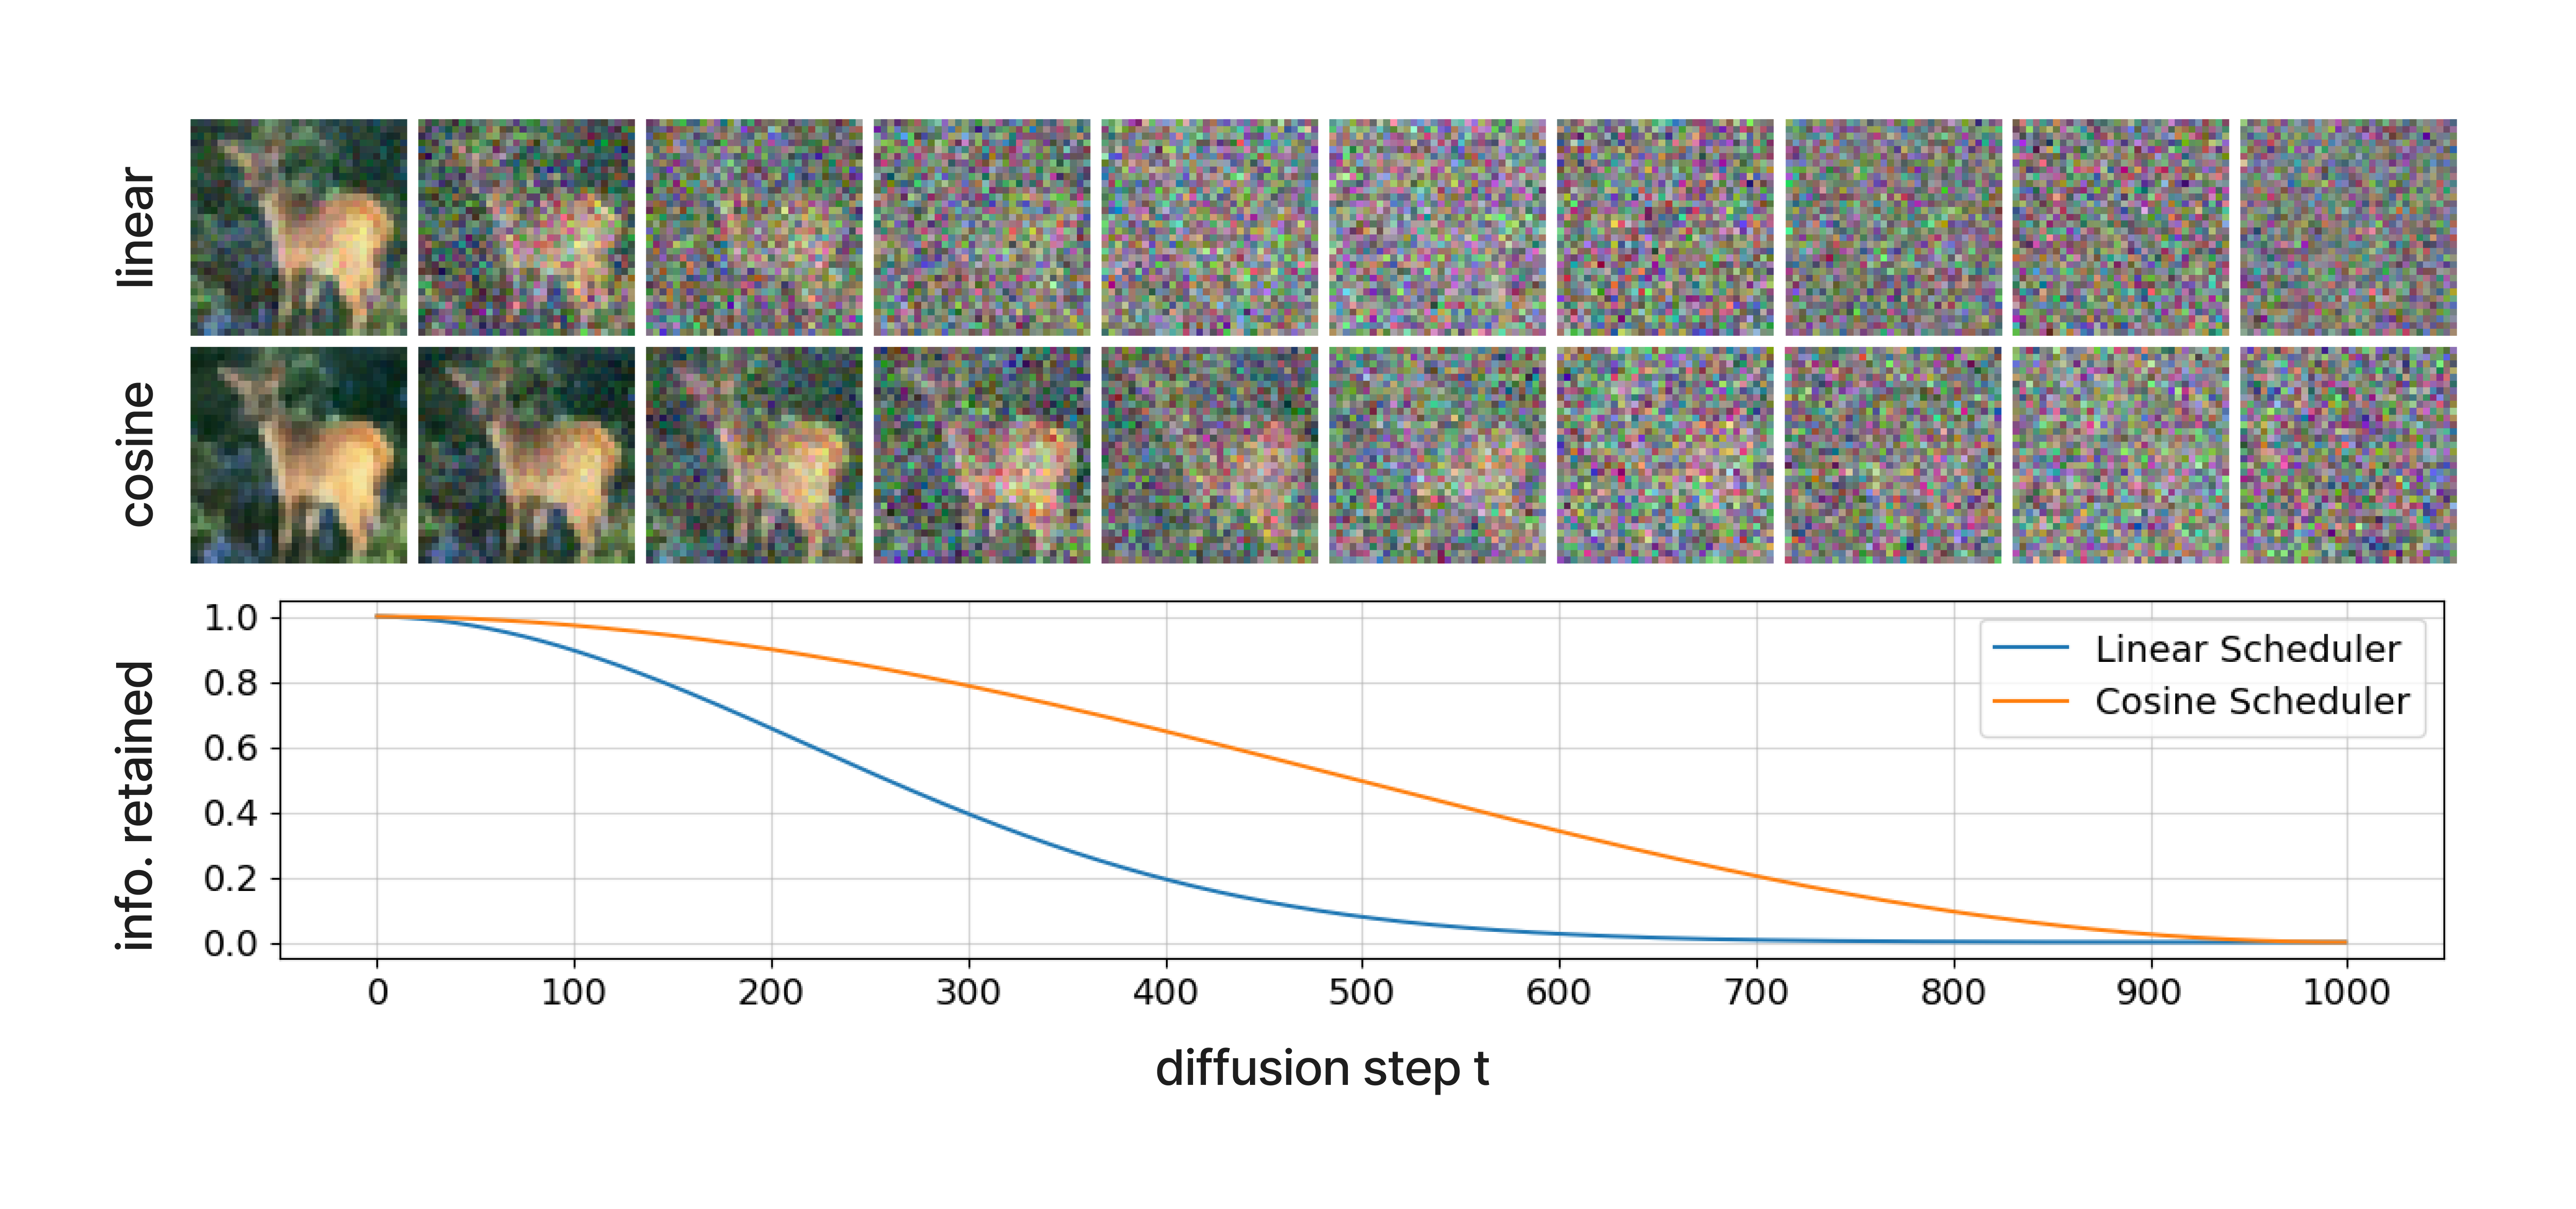
\includegraphics[width=0.8\textwidth]{figs/noise_decay.png}
					\caption{Visualization of Noise Decay over Time}
					\label{fig:noise_decay}
				\end{figure}

			\end{block}

			\begin{block}{Reducing Gradient Noise}
				\begin{columns}
					\begin{column}{0.4\textwidth}
						\begin{center}
							% \begin{figure}
							% 	\begin{tikzpicture}
							% 		\begin{axis}[
							% 				scale only axis,
							% 				no markers,
							% 				domain=0:2*pi,
							% 				samples=100,
							% 				axis lines=center,
							% 				axis line style={-},
							% 				ticks=none]
							% 			\addplot[red] {sin(deg(x))};
							% 			\addplot[blue] {cos(deg(x))};
							% 		\end{axis}
							% 	\end{tikzpicture}
							% 	\caption{Another figure caption.}
							% \end{figure}
							
							\begin{table}[h]
								\centering
								\begin{tabular}{llcc}
									\toprule
									\textbf{Objective} & \textbf{Schedule} & \textbf{NLL} & \textbf{FID} \\
									\midrule
									$L_{\text{simple}}$ & linear  & 3.80  & 9.03  \\
									$L_{\text{simple}}$ & cosine  & 3.57  & \textbf{7.28}  \\
									$L_{\text{vlb}}$    & linear  & 3.62  & 26.75 \\
									$L_{\text{vlb}}$ (sampled) & linear  & \textbf{3.45}  & 25.29 \\
									$L_{\text{hybrid}}$ & \textbf{linear} & \textbf{3.59}  & 9.35  \\
									\bottomrule
								\end{tabular}
								\caption{Comparison of different objectives and schedules in terms of NLL and FID.}
								\label{tab:results}
							\end{table}

						\end{center}
					\end{column}
					\begin{column}{0.6\textwidth}  %%<--- here
						\justify
						Lorem ipsum dolor sit amet, consectetur adipiscing elit. Aliquam vel dapibus erat. Morbi quis leo congue, lobortis augue bibendum, malesuada neque. Duis ullamcorper quis orci sed consequat. Nam pellentesque ullamcorper tempor. Duis eget nulla blandit, vulputate orci vitae, ullamcorper ligula. Mauris a urna ac massa dignissim scelerisque sed et augue. Donec eget urna vitae neque elementum pellentesque et eget enim. Praesent a fermentum nibh. Nullam eu nibh neque.
					\end{column}
				\end{columns}


			\end{block}

			\begin{block}{Improving Sampling Speed}

				Nulla eget sem quam. Ut aliquam volutpat nisi vestibulum convallis. Nunc a
				lectus et eros facilisis hendrerit eu non urna. Interdum et malesuada fames
				ac ante \textit{ipsum primis} in faucibus. Etiam sit amet velit eget sem
				euismod tristique. Praesent enim erat, porta vel mattis sed, pharetra sed
				ipsum. Morbi commodo condimentum massa, \textit{tempus venenatis} massa
				hendrerit quis. Maecenas sed porta est. Praesent mollis interdum lectus,
				sit amet sollicitudin risus tincidunt non.

			\end{block}

		\end{column}

		\separatorcolumn

		\begin{column}{\colwidth}

			\begin{exampleblock}{A highlighted block containing some math}

				A different kind of highlighted block.

				$$
					\int_{-\infty}^{\infty} e^{-x^2}\,dx = \sqrt{\pi}
				$$

				Interdum et malesuada fames $\{1, 4, 9, \ldots\}$ ac ante ipsum primis in
				faucibus. Cras eleifend dolor eu nulla suscipit suscipit. Sed lobortis non
				felis id vulputate.

			\end{exampleblock}

			\begin{block}{Interpolation \& Latent Conditional Sampling}
				We take two source images $x_0, x_{0}^{'} \sim q(x_0)$ and interpolate their latent space representations using $q$ as a stochastic encoder,  $x_t, x_{t}^{'} \sim q(x_t \mid x_0)$, then decoding the linearly interpolated latent $\bar{x}_{0} = (1 - \lambda)x_{0} + \lambda x_{0}^{'}$ into image space by the reverse process, $\bar{x}_{0} \sim p(x_{0} \mid \bar{x}_{t})$. The reverse process produces high-quality reconstructions and plausible interpolations that smoothly vary various attributes.

				\begin{figure}[h]
					\centering
					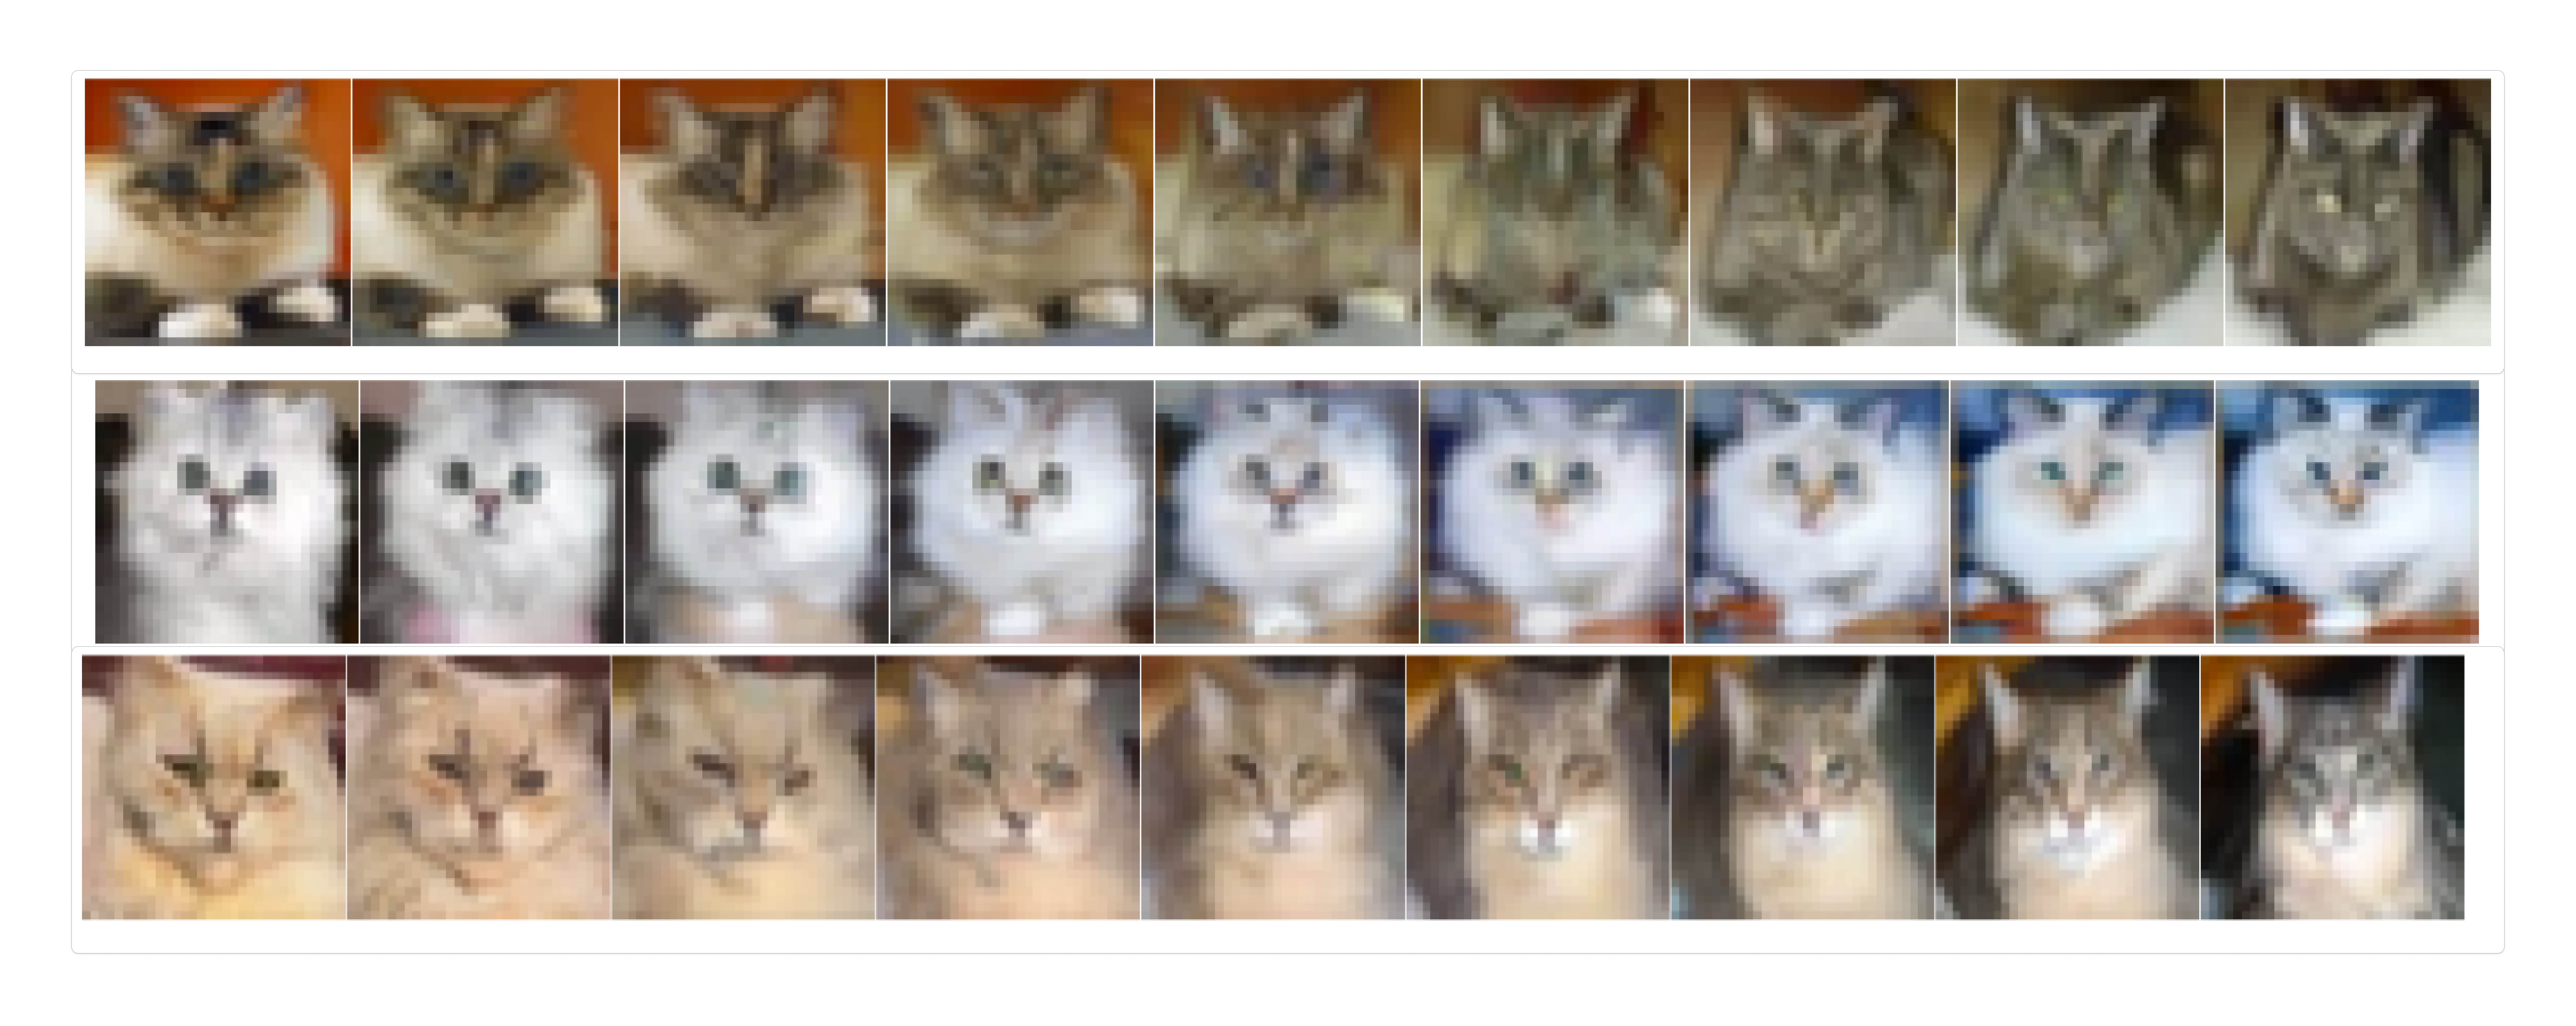
\includegraphics[width=0.8\textwidth]{figs/interpolation.png}
					\caption{Latent State Interpolation}
					\label{fig:interpolation}
				\end{figure}
				
				\begin{figure}[h]
					\centering
					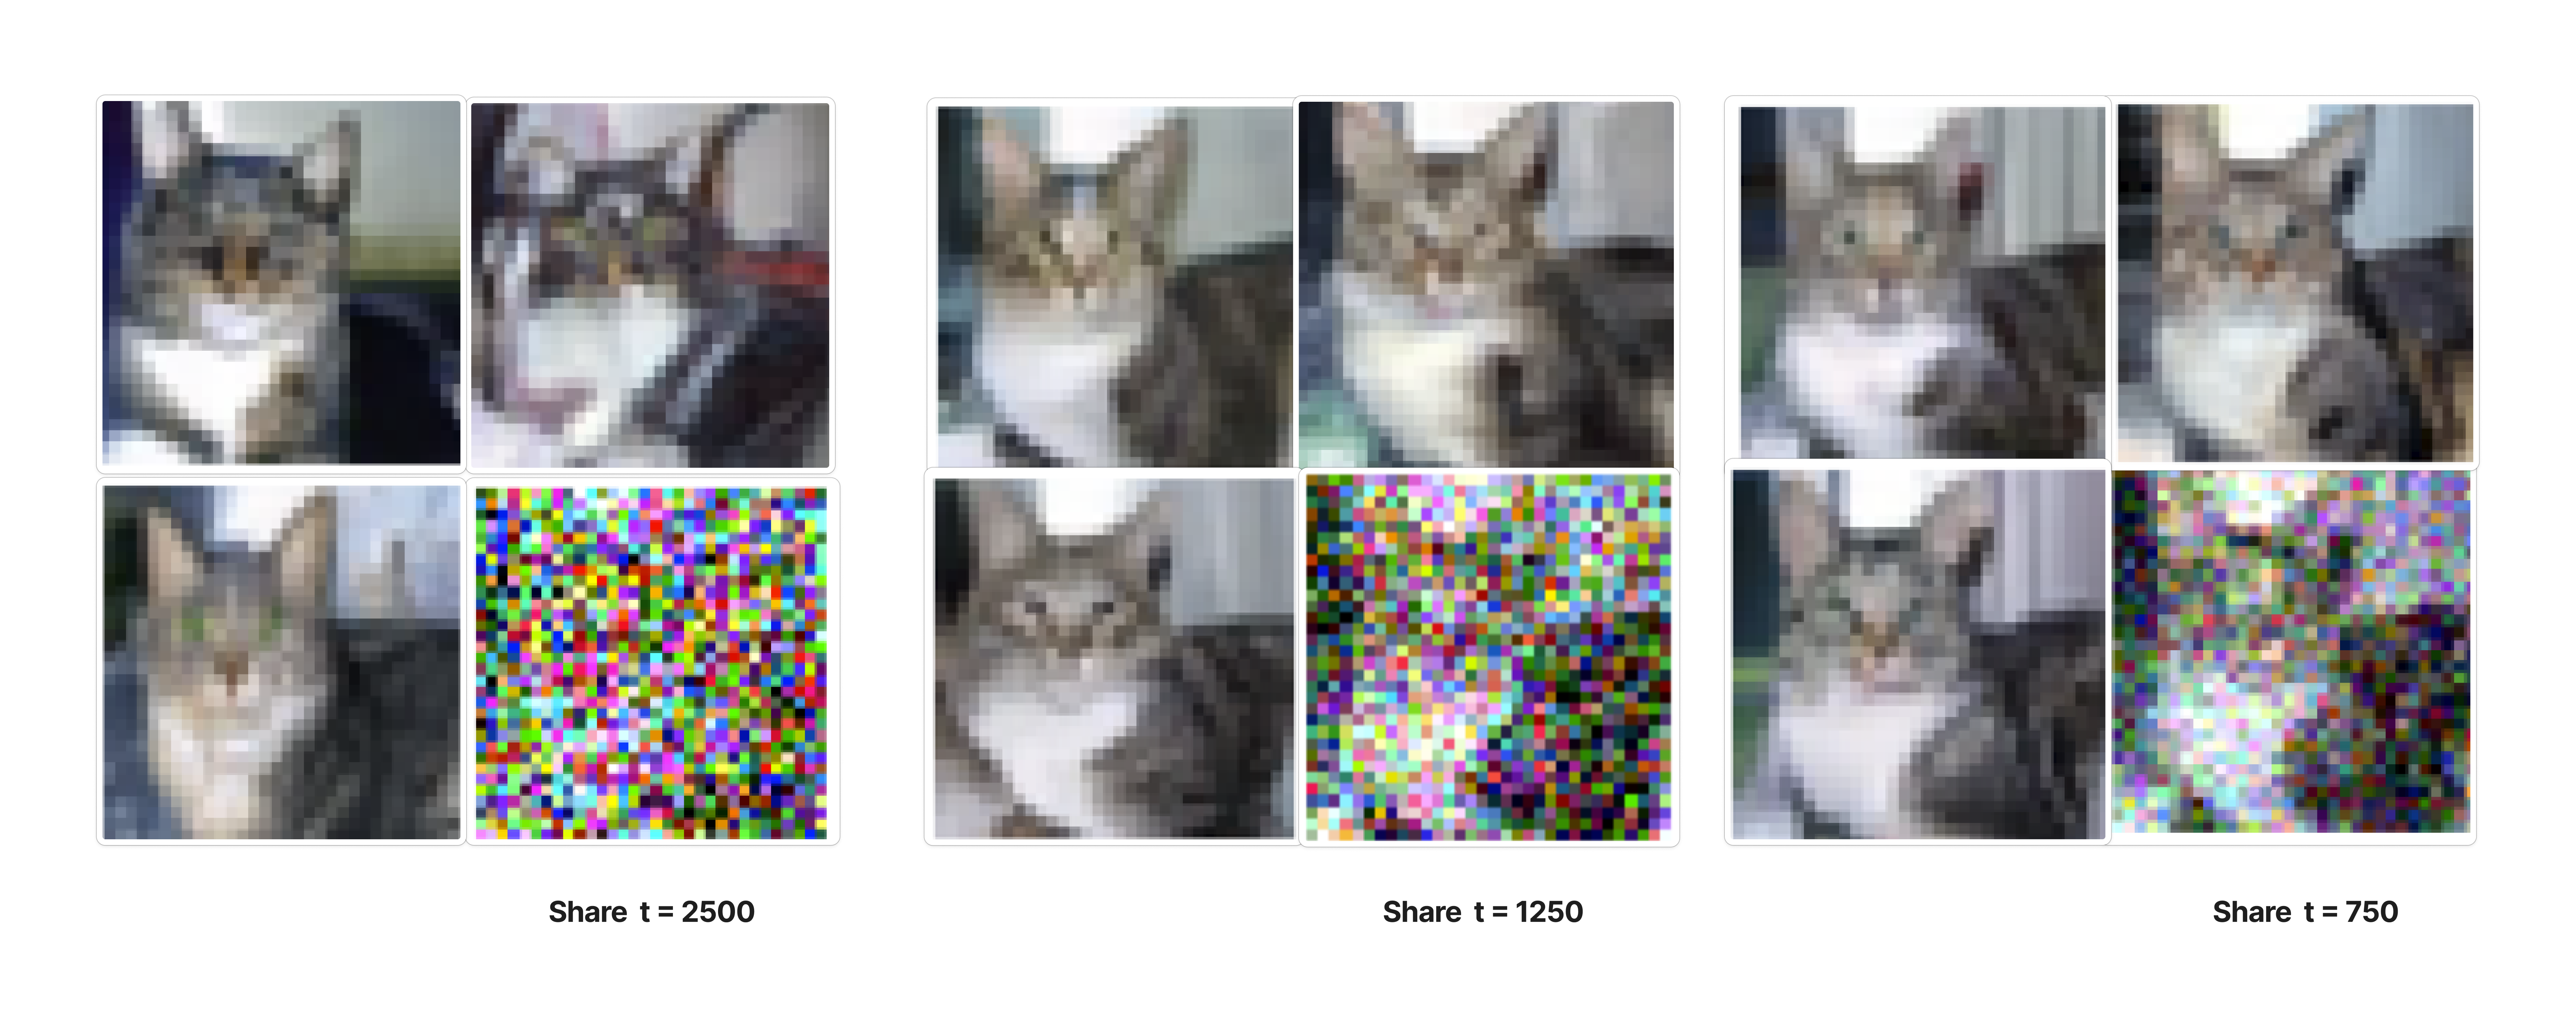
\includegraphics[width=0.8\textwidth]{figs/latent_conditional.png}
					\caption{Latent Conditional Sampling}
					\label{fig:latent_conditional}
				\end{figure}
				
			\end{block}

			\begin{block}{References}

				\nocite{*}
				\footnotesize{\bibliographystyle{plainnat}\bibliography{poster}}

			\end{block}

		\end{column}

		\separatorcolumn
	\end{columns}
\end{frame}

\end{document}
